\documentclass[12pt,a4paper]{article}

% ---------------------------------------------------------------
%  NOGA 2027 Call for Research Proposals
%  Research domain 2.5 -- Forming the demand forecast of the
%  electricity system (with links to 2.1.5, 2.2.2, 2.1.6, 2.4.3).
%  Language: English.  Font: 12pt.  Page: A4.  Pages numbered.
% ---------------------------------------------------------------

\usepackage[T1]{fontenc}
\usepackage[utf8]{inputenc}
\usepackage{lmodern}
\usepackage{graphicx}
\usepackage{amsmath}
\usepackage{amssymb}
\usepackage[margin=1.1in]{geometry}
\usepackage[hidelinks]{hyperref}
\usepackage{placeins}
\usepackage{float}
\usepackage{booktabs}
\usepackage{array}
\usepackage{caption}
\usepackage{subcaption}
\usepackage{setspace}
\usepackage{parskip}
\usepackage{microtype}
\usepackage{xcolor}
\usepackage{colortbl}
\usepackage{enumitem}
\usepackage{titlesec}
\usepackage{fancyhdr}
\usepackage{pgfgantt}
\usepackage[style=authoryear,backend=biber,maxbibnames=8,sorting=nyt]{biblatex}

\emergencystretch=1em
\addbibresource{ref.bib}
\onehalfspacing

% --- light section styling for a clean proposal look ---
\definecolor{nogablue}{RGB}{0,76,140}
\titleformat{\section}{\Large\bfseries\color{nogablue}}{\thesection}{0.6em}{}
\titleformat{\subsection}{\large\bfseries\color{nogablue!85!black}}{\thesubsection}{0.6em}{}
\titleformat{\subsubsection}{\normalsize\bfseries}{\thesubsubsection}{0.6em}{}

% --- header / footer with page numbers (required) ---
\setlength{\headheight}{14.5pt}
\addtolength{\topmargin}{-2.5pt}
\pagestyle{fancy}
\fancyhf{}
\renewcommand{\headrulewidth}{0.4pt}
\lhead{\small Probabilistic Net-Demand Forecasting}
\rhead{\small NOGA R\&D 2027}
\cfoot{\thepage}

\newcommand{\domain}[1]{\textcolor{nogablue}{\textbf{#1}}}

\begin{document}

% ===============================================================
%  TITLE PAGE  (Appendix A, sec. 2.1)
% ===============================================================
\thispagestyle{empty}
\begingroup
\singlespacing
\begin{center}
    \vspace*{0.2cm}
    {\large\bfseries Research Proposal submitted to}\\[0.2em]
    {\large NOGA -- Israel Independent System Operator}\\[0.3em]
    {\normalsize Call for Research Proposals for 2027 in the Fields of the Electricity System}\\[0.9cm]

    \rule{\textwidth}{1.2pt}\\[0.5cm]
    {\LARGE\bfseries\color{nogablue}
     Integrated Probabilistic Forecasting of\\[0.25em]
     Electricity Demand and Renewable Generation\\[0.25em]
     for Risk-Aware Grid Operation\par}
    \vspace{0.4cm}
    {\large\itshape From Cost-Sensitive Point Forecasts to\\
     Calibrated Predictive Distributions}\\[0.35cm]
    \rule{\textwidth}{1.2pt}\\[0.9cm]

    \begin{tabular}{rl}
        \textbf{Principal Researcher:} & [Name] \\[0.35em]
        \textbf{Co-Researchers:}       & [Names of co-Researchers --- placeholder] \\[0.35em]
        \textbf{Institution:}            & Technion --- Israel Institute of Technology \\[0.35em]
        \textbf{Faculty / Department:}   & [Faculty --- placeholder] \\[0.35em]
        \textbf{Partner bodies:}         & NOGA --- Israel ISO (data \& domain collaboration) \\[0.35em]
        \textbf{Contact:}                & gilad.kutiel@gmail.com \\[0.35em]
    \end{tabular}

    \vspace{0.9cm}
    \begin{tabular}{rl}
        \textbf{Primary research domain:} & 2.5 --- Forming the Demand Forecast of the \\
                                          & \phantom{2.5 --- }Electricity System (\S2.5.1, \S2.5.2) \\[0.35em]
        \textbf{Secondary domains:}       & 2.2.2 (monitoring \& state forecasting),\\
                                          & 2.1.5 (stability \& ancillary services / reserve),\\
                                          & 2.1.6 (sustainable / renewable integration),\\
                                          & 2.4.3 (operation under limited reserves) \\[0.35em]
        \textbf{Proposed duration:}       & 36 months (submitted annually) \\[0.35em]
        \textbf{Date of submission:}      & June 2026 \\
    \end{tabular}
\end{center}
\endgroup
\newpage

% ===============================================================
%  ABSTRACT  (Appendix A, sec. 2.2 -- up to half a page)
% ===============================================================
\section*{Abstract}
\addcontentsline{toc}{section}{Abstract}

Accurate demand forecasting underpins the safe and economic operation of the power
system: procurement and reserve decisions are committed before demand and renewable
generation are observed. Operational forecasts today are predominantly \emph{point}
forecasts trained on symmetric losses (e.g.\ MSE), implicitly treating over- and
under-supply as equally costly. In reality these costs are strongly asymmetric and
state-dependent---governed by reserve availability, volatile solar and wind output,
real-time energy prices, and penalties for unserved load.

\paragraph{The goal} is to move from point forecasts to \emph{calibrated predictive
distributions}: advanced probabilistic techniques that output the full conditional
distribution of (i)~national demand and (ii)~renewable generation, \emph{integrated} into
a coherent forecast of \emph{net demand} (residual load), with a decision layer that
converts these distributions into cost- and risk-optimal reserve and procurement quantities.

\paragraph{Methodologically}, we develop and compare techniques that produce calibrated
distributions with finite-sample reliability guarantees, integrate the demand and renewable
distributions while respecting their statistical dependence, and evaluate them with proper
scoring rules and---crucially---\emph{operational cost}. The work builds on our preliminary
results, in which cost-aware training on three years of real NOGA and Israel Meteorological
Service data cut operational cost by 40--73\% over symmetric baselines.

\paragraph{Expected outcomes} are an open, reproducible probabilistic forecasting framework
for the Israeli grid, quantified reliability and cost improvements over the current
operational forecast, and a deployable decision tool for risk-aware reserve sizing. The
proposal directly addresses NOGA R\&D domain~\textbf{2.5} and supports reserve, stability,
and renewable-integration objectives (\S2.1.5, \S2.2.2, \S2.1.6).

\paragraph{Beneficiaries.} \textbf{NOGA} gains sharper, risk-aware day-ahead and intraday
decisions driven by a calibrated net-demand distribution rather than a cost-blind point
forecast; \textbf{electricity suppliers and traders} obtain better-quantified uncertainty
for smarter procurement and bidding; \textbf{consumers} benefit from the lower system costs
and higher reliability of leaner, better-targeted reserves; and \textbf{the research
community} gains an open benchmark for probabilistic net-demand forecasting on a real
national grid, with peer-reviewed publications.

\newpage

% ===============================================================
%  TABLE OF CONTENTS  (Appendix A, sec. 2.3)
% ===============================================================
\tableofcontents
\newpage

% ===============================================================
%  RESEARCH DESCRIPTION  (Appendix A, sec. 2.4)
% ===============================================================
\section{Introduction}
\label{sec:intro}

\subsection{Background and Motivation}

The Israeli power system, operated by NOGA, must continuously balance supply and demand
under tight reliability constraints and a rapidly changing generation mix. Day-ahead and
intraday scheduling, reserve allocation, and unit commitment all depend on a forecast of
how much electricity will be consumed---and, increasingly, on how much will be supplied
by weather-driven renewable sources whose output the operator does not control. As the
share of distributed solar photovoltaics (PV) and other variable renewables grows, the
quantity that actually governs operational risk is no longer gross demand but
\emph{net demand} (residual load): demand minus renewable generation. Net demand is more
volatile and less predictable, exhibiting steep ramps and pronounced troughs as variable
generation rises and falls against an already fluctuating load
\parencite{denholm2015overgeneration}. Forecasting it well is
central to maintaining adequate operating reserves, avoiding both shortfalls and costly
over-generation, and integrating renewables without compromising reliability.

Both sides of this balance are shaped by distinctly local conditions. On the demand side,
domestic consumption fluctuates on daily and weekly cycles that follow varying personal
habits, and it is distributed unevenly across the grid because of geographic and
socio-economic differences between consumers. Israel makes this heterogeneity acute:
despite its small area it spans four distinct climatic zones, and its four main urban
concentrations---Jerusalem, the Tel~Aviv metropolitan area, Haifa, and Be'er~Sheva---differ
markedly in population composition and consumption patterns. Compounding this, the Israeli
load relies heavily on electric HVAC for both heating and cooling, so the magnitude and
volatility of demand peaks are tied directly to weather, and not only to human routine.
This places weather forecasting at the heart of demand forecasting---yet urban weather
prediction is inherently inaccurate for two reasons. First, hourly air temperature and
relative humidity are intrinsically hard to predict at fine geographic resolution. Second,
the standard practice of forecasting from non-urban monitoring stations ignores the urban
heat island effect---the additional warming generated by the built environment---precisely
where load is concentrated.

A central and under-exploited fact is that the cost of a forecast error is strongly
\emph{asymmetric} and \emph{state-dependent}. When the system under-provisions---demand
exceeds the committed supply, or renewables under-deliver---the operator must activate
expensive fast reserves, purchase energy in a volatile real-time market, or, in the
extreme, shed load; the per-unit cost can be several multiples of the day-ahead price and
carries reliability and regulatory consequences \parencite{stoft2002power}. When the
system over-provisions, the surplus is curtailed, exported, or stored at a comparatively
modest and bounded cost. Empirically, the ratio of under- to over-provisioning cost in
electricity markets typically lies in the range $[5,20]$
\parencite{zhang2022costoriented}. This asymmetry means that the operationally optimal
forecast is \emph{not} the conditional mean (the target of MSE-trained models) but a
deliberately biased quantile of the demand distribution---and, more generally, a quantity
derived from the \emph{full predictive distribution} of net demand.

\subsection{The Limits of Point Forecasting}
\label{sec:limits}

Despite this, the forecasts used operationally---including, as our preliminary analysis
shows, the current NOGA day-ahead forecast---behave as accurate but essentially
\emph{cost-blind} conditional-mean estimators (Section~\ref{sec:prelim}). A single point
forecast, however accurate in MSE terms, discards exactly the information an operator
needs to make a risk-aware decision: how uncertain is the forecast \emph{right now}, how
heavy are the tails, and how should the procurement quantity shift as the cost of a
shortfall rises or as reserve margins tighten? Two forecasts with identical point values
but different uncertainty warrant different reserve commitments. Point forecasting cannot
express this distinction.

The natural remedy is \emph{probabilistic forecasting}: predicting the full conditional
distribution of the target rather than a single value \parencite{gneiting2014probabilistic,
hong2016probabilistic}. A predictive distribution allows the operator to (i)~select the
cost-optimal procurement quantile for \emph{any} cost asymmetry without retraining;
(ii)~quantify the probability and expected magnitude of a shortfall (value-at-risk,
expected shortfall); and (iii)~size reserves to a chosen reliability target. When the
distributions of demand \emph{and} renewable generation are available and correctly
\emph{coupled}, the operator obtains a distribution of net demand---the quantity that
actually drives reserve and balancing decisions.

\subsection{Related Work}
\label{sec:related}

\paragraph{Asymmetric loss and quantile estimation.}
The decision-theoretic foundation for forecasting under asymmetric costs was established
by \textcite{christoffersen1997optimal}, who showed that under a general asymmetric loss
the optimal point forecast is biased by an amount that depends on conditional higher-order
moments---so any symmetric-loss forecast is systematically suboptimal when costs are
asymmetric. \textcite{koenker1978regression} introduced regression quantiles and the
pinball (``check'') loss, whose minimiser is the conditional quantile; this underpins
modern quantile forecasting. The classical newsvendor model
\parencite{arrow1951optimal} gives the corresponding closed form: under linear costs the
optimal procurement level is the $c_u/(c_u+c_o)$ quantile of demand.

\paragraph{Cost-oriented and probabilistic load forecasting.}
A growing literature embeds operational cost into the learning objective.
\textcite{wang2019pinball} train an LSTM with pinball loss for probabilistic individual
load forecasting; \textcite{lin2020asymmetric} derive asymmetric losses from a utility's
tariff and reduce cost by up to 2.4\%; \textcite{wu2021svr} obtain large economic
savings with an asymmetric support-vector formulation; and
\textcite{zhang2022costoriented} formalise ``cost-oriented'' load forecasting that scores
forecasts by downstream operating cost rather than statistical error. On the
distributional side, \textcite{hong2016probabilistic} review probabilistic load
forecasting and argue that point forecasts are insufficient for operational
decision-making; GEFCom2014 \parencite{hong2016gefcom2014} established the pinball loss
and full predictive quantiles as community standards; and \textcite{salinas2020deepar}
demonstrate scalable autoregressive deep probabilistic forecasting. Methodologically,
modern deep models can represent rich predictive densities via normalizing flows
\parencite{rezende2015variational,papamakarios2021normalizing} or deep ensembles
\parencite{lakshminarayanan2017simple}, and conformal prediction
\parencite{vovk2005algorithmic,romano2019conformalized} supplies finite-sample coverage
guarantees that pure deep models lack. The quality of a probabilistic forecast is judged
by strictly proper scoring rules such as the CRPS \parencite{gneiting2007strictly}.

\paragraph{Renewable forecasting and operating reserve.}
Probabilistic forecasting of solar PV and wind is a mature field
\parencite{antonanzas2016review,hong2020energy}, and methods exist to convert marginal
probabilistic forecasts into temporally coherent scenarios via copulas
\parencite{pinson2009scenarios,nelsen2006copulas}. On the decision side,
\textcite{matos2011reserve} show how to set operating reserve directly from probabilistic
wind forecasts, and \textcite{morales2014integrating} develop the broader theory of
operating power systems with high renewable penetration under uncertainty.

\subsection{Research Gap and Problem Statement}
\label{sec:gap}

Three gaps remain, and together they define this proposal. \emph{First}, the cost-oriented
forecasting literature largely produces a \emph{single} cost-tuned point (or a fixed set
of quantiles); it does not deliver a calibrated full distribution from which \emph{any}
cost-optimal decision can be read off as the cost structure changes. \emph{Second}, demand
forecasting and renewable forecasting are typically studied in isolation, whereas the
operationally decisive quantity is their \emph{coupled} net demand, whose distribution
depends on the statistical dependence between load and weather-driven generation.
\emph{Third}, very little of this work is grounded in, or validated against, the
\emph{real operational forecast} of a system operator on a specific national grid.

\medskip\noindent\textbf{Problem statement.} \emph{Given historical demand, renewable
generation, weather, and calendar information for the Israeli grid, learn calibrated
conditional predictive distributions of demand and of renewable generation; couple them
into a predictive distribution of net demand; and from this distribution compute reserve
and procurement decisions that minimise expected operational cost and control the risk of
shortfall---demonstrably improving on the current operational point forecast.}

\subsection{Preliminary Results}
\label{sec:prelim}

This proposal is a direct, evidence-backed extension of work the research team has already carried
out. We assembled a dataset spanning \textbf{March~2023--February~2026} (1{,}096 days)
combining real NOGA demand readings \emph{and the actual day-ahead operational forecasts}
with Israel Meteorological Service weather data (temperature, humidity, wind) from
Tel~Aviv, Jerusalem, and Haifa \parencite{noga,ims}. On this dataset we established two
findings that motivate the present proposal.

\paragraph{(1) The operational forecast is accurate but cost-blind.}
The NOGA day-ahead forecast achieves $R^2\approx 0.98$ and is nearly unbiased: its error
distribution is approximately zero-mean and symmetric (mean $+312$~MWh against a standard
deviation of $3{,}241$~MWh; Figure~\ref{fig:kde}). This is excellent from an accuracy
standpoint but, under asymmetric costs, it is precisely the wrong target---a symmetric,
mean-unbiased forecast systematically under-provisions relative to the cost-minimising
quantile.

\paragraph{(2) Cost-aware training yields large operational gains.}
We trained neural forecasters with cost-sensitive (asymmetric-loss) objectives at
under/over cost ratios of $5\!:\!1$ and $20\!:\!1$ and compared them with a symmetric baseline and
with post-hoc affine calibration. Cost-aware training reduced operational cost by
\textbf{40\%} at a $5\!:\!1$ ratio and by \textbf{73\%} at a $20\!:\!1$ ratio relative to
the symmetric baseline (Figure~\ref{fig:confusion}), with the error distribution shifting
exactly as theory predicts (Figure~\ref{fig:histograms}). Critically, post-hoc affine
calibration narrowed but did \emph{not} close the gap, because a single global correction
cannot reproduce the \emph{input-conditional} adjustment---larger when uncertainty and
shortfall risk are higher---that end-to-end training learns. This is direct empirical
evidence that the \emph{shape} of the conditional distribution, not just a global offset,
carries operational value: exactly the object this proposal sets out to model in full.

\begin{figure}[H]
    \centering
    \begin{subfigure}[t]{\linewidth}
        \centering
        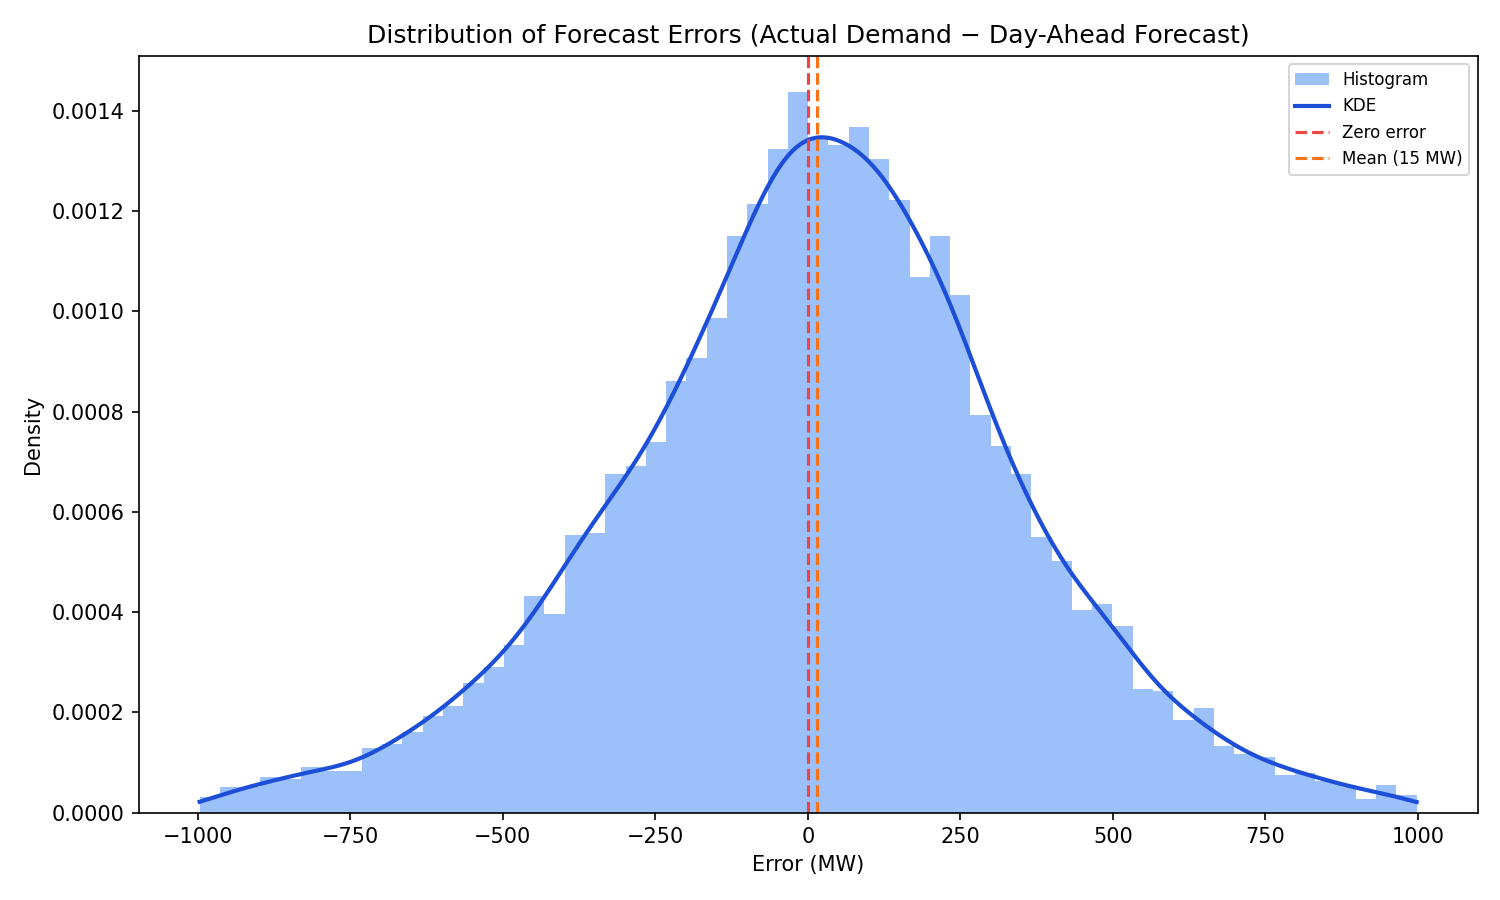
\includegraphics[width=\linewidth]{plot/demand_vs_forecast_kde_histogram.png}
        \caption{NOGA day-ahead forecast error (actual minus forecast). Nearly
                 zero-mean and symmetric: accurate, but blind to cost asymmetry.}
        \label{fig:kde}
    \end{subfigure}

    \vspace{0.8em}
    \begin{subfigure}[t]{\linewidth}
        \centering
        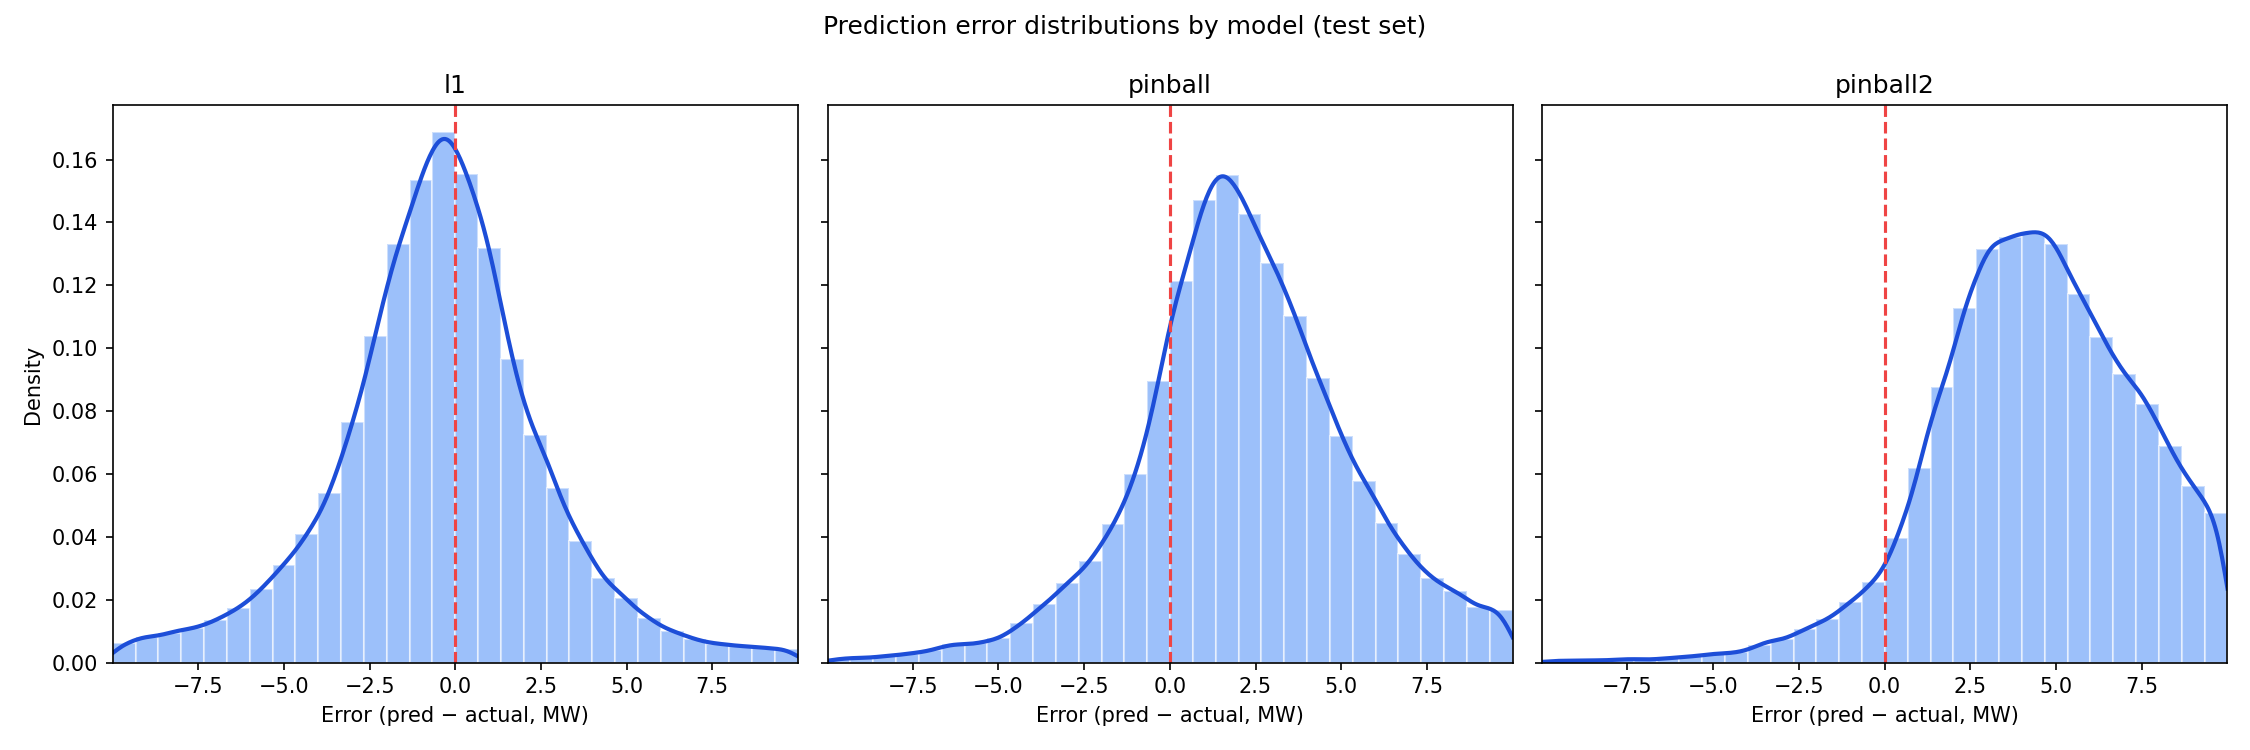
\includegraphics[width=\linewidth]{plot/error_histograms.png}
        \caption{Test-set error distributions of cost-aware models. Higher cost
                 ratios induce a deliberate, larger upward shift.}
        \label{fig:histograms}
    \end{subfigure}
    \caption{Preliminary results (current project): the operational forecast behaves as a
             cost-blind conditional-mean estimator (top), whereas cost-aware training
             reshapes the predictive response (bottom).}
    \label{fig:prelim-pair}
\end{figure}

\begin{figure}[H]
    \centering
    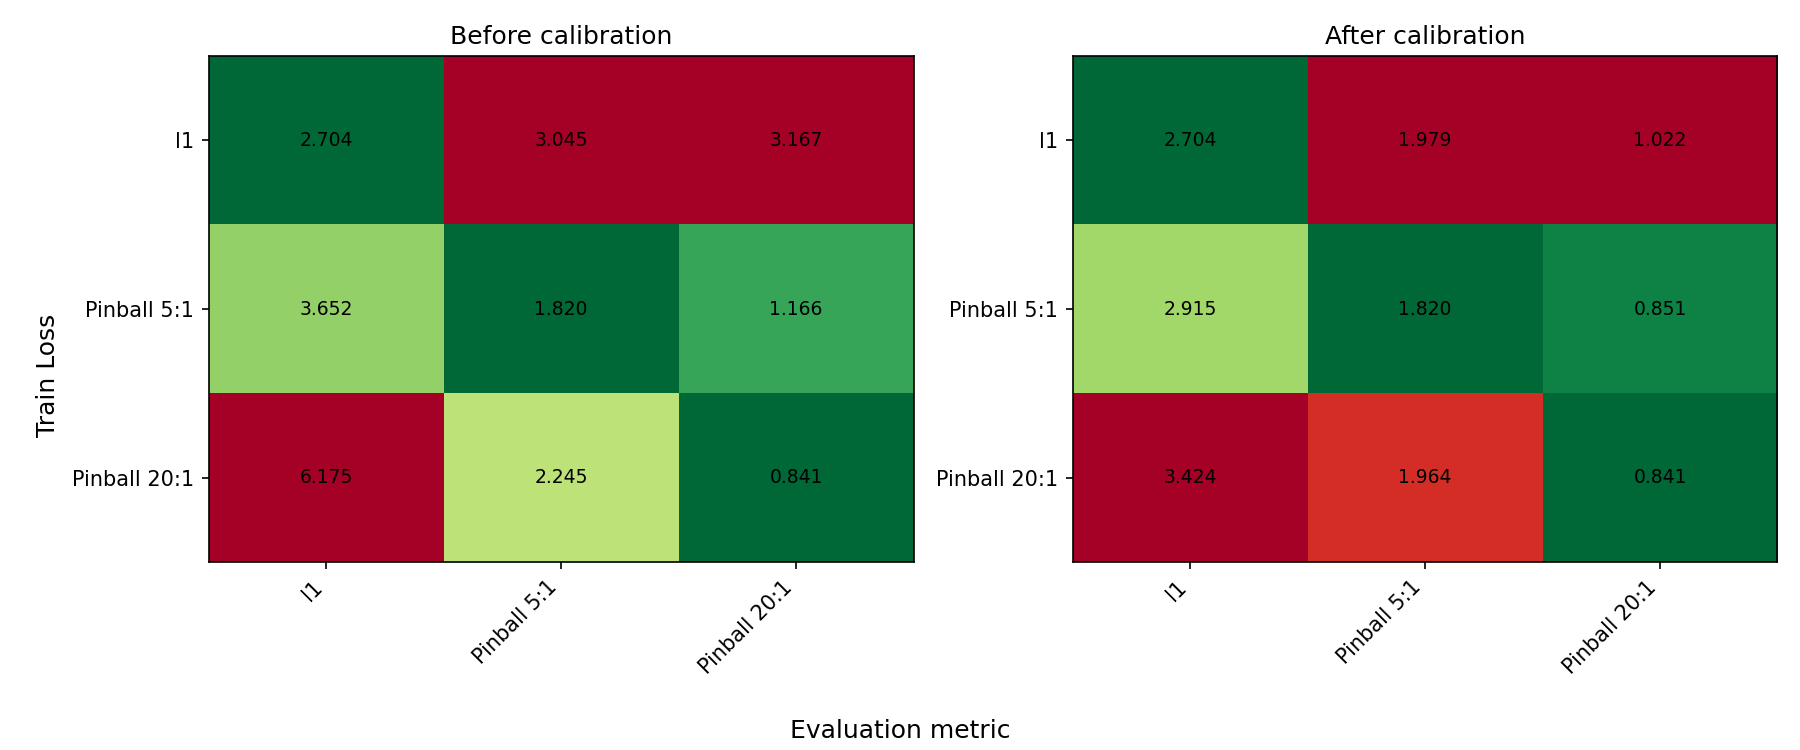
\includegraphics[width=\linewidth]{plot/confusion_matrix.png}
    \caption{Preliminary results: training-loss $\times$ evaluation-metric cost matrix
             (lower is better; green best, red worst). Each model wins on the metric it was
             trained for; cost-aware models cut operational cost by 40--73\% over the
             symmetric baseline, and post-hoc calibration (right) does not fully recover
             the gap. This motivates modelling the \emph{full} predictive distribution.}
    \label{fig:confusion}
\end{figure}

These results de-risk the proposal: the data pipeline, the real operational baseline, and
the cost-evaluation methodology already exist. What remains---and what we propose---is the
scientifically substantial step from a single cost-tuned quantile to a calibrated,
\emph{integrated} predictive distribution of demand and renewable generation, with an
explicit decision layer.

% ===============================================================
\section{Research Tasks}
\label{sec:objectives}

The overarching aim is to develop and validate, on the Israeli grid, an integrated
probabilistic forecasting and decision framework for net demand. This decomposes into five
specific tasks:

\begin{description}[leftmargin=2.2em,style=nextline]
    \item[\textbf{T1. Extended dataset \& open benchmark.}] Augment the existing
        demand--weather dataset with renewable-generation data (system-level solar PV and
        wind, with distributed-PV estimation), reserve/balancing indicators, and calendar
        and special-day features, and release a reproducible benchmark for probabilistic
        net-demand forecasting on the Israeli grid.
    \item[\textbf{T2. Calibrated probabilistic demand forecasting.}] Develop and compare
        advanced probabilistic forecasting techniques that output the full conditional
        distribution of demand, calibrated to finite-sample coverage guarantees, across
        day-ahead and intraday horizons.
    \item[\textbf{T3. Probabilistic renewable-generation forecasting.}] Develop analogous
        predictive distributions for renewable generation, capturing the non-Gaussian,
        bounded, weather-driven and strongly diurnal/seasonal behaviour of PV and wind.
    \item[\textbf{T4. Integration into a net-demand distribution.}] Couple the demand and
        renewable predictive distributions---explicitly modelling their statistical
        dependence---to obtain a calibrated predictive distribution of net demand and
        temporally coherent scenarios.
    \item[\textbf{T5. Risk-aware decision layer and operational validation.}] Convert the
        net-demand distribution into cost-optimal reserve and procurement decisions under
        general (possibly state-dependent) asymmetric costs, quantify reliability and cost
        improvements over the current NOGA operational forecast, and deliver a deployable
        prototype with knowledge transfer to NOGA.
\end{description}

% ===============================================================
\section{Methodology}
\label{sec:methodology}

\subsection{Research Design and Overall Approach}

We adopt a modular pipeline---\emph{data $\rightarrow$ distributional demand model
$\rightarrow$ distributional renewable model $\rightarrow$ coupling $\rightarrow$ decision
layer}---in which each stage is independently testable and reuses the validated
infrastructure from our preliminary work. Development is incremental: each probabilistic
component is first benchmarked against the corresponding point forecaster and the NOGA
operational baseline before integration, so that scientific risk is contained at each
step (Section~\ref{sec:risks}). All models are trained and evaluated with strictly
chronological splits to prevent information leakage, mirroring true operational deployment.

\subsection{Data Collection and Preparation (T1)}
\label{sec:data}

The foundation is the existing three-year dataset of NOGA demand, the real NOGA day-ahead
forecast, and IMS weather for the three principal load centres
\parencite{noga,ims}. We will extend it along three axes:
\begin{itemize}[leftmargin=1.4em]
    \item \textbf{Renewable generation:} system-level PV and wind generation and
        installed capacity; where distributed (``behind-the-meter'') PV is only implicitly
        observable, we will estimate it from irradiance/temperature proxies and the
        demand signal, an established practice in net-load studies.
    \item \textbf{Operational/market context:} reserve margins, balancing actions and any
        available cost/price proxies, to ground the cost model of Task~T5 in
        operational reality rather than purely synthetic costs.
    \item \textbf{Exogenous drivers:} richer weather inputs---solar irradiance (measured
        directly at only a handful of stations in Israel, so cloud cover must be inferred
        from it rather than measured), air temperature (which lowers PV panel efficiency as
        it rises), wind, and additional stations---together with calendar effects, holidays
        and special days, which are known to drive the hardest-to-forecast slots in our
        preliminary error analysis. Where possible we will also ingest real-time
        observations through the IMS data API.
\end{itemize}
The result will be released, to the extent permitted by data agreements, as an open
benchmark with fixed splits and baseline scripts---a contribution in its own right and a
prerequisite for reproducible evaluation.

\subsection{Calibrated Probabilistic Demand Forecasting (T2)}
\label{sec:demand}

Let $x_t$ denote the feature vector available at decision time for target time $t$
(recent demand, weather, calendar embeddings, as in our current architecture). We seek the
full conditional distribution $F_{D}(\cdot \mid x_t)$ of demand $D_t$, rather than a single
point estimate. We will develop and systematically compare a range of \emph{advanced
probabilistic forecasting techniques} that represent this conditional distribution with
increasing flexibility---from techniques that predict a set of conditional quantiles,
through those that predict the parameters of a flexible density, to fully non-parametric
techniques able to capture skew, heavy tails, and multimodality. All variants generalise
our current cost-sensitive model, are trained end-to-end, and are benchmarked under a
single protocol against the operational baseline.

Because flexible models are frequently mis-calibrated, every technique will be wrapped in
a distribution-free \textbf{calibration} layer that provides finite-sample coverage
guarantees---a property of direct operational importance when reserves are sized to a
target reliability level. Models will be scored by proper scoring rules, by empirical
coverage/reliability, and---decisively---by downstream operational cost, reusing the
evaluation machinery validated in our preliminary work.

\subsection{Probabilistic Renewable-Generation Forecasting (T3)}
\label{sec:renewable}

Renewable generation is bounded (non-negative, capacity-capped), strongly diurnal and
seasonal, and highly weather-sensitive, so its predictive density is far from Gaussian
\parencite{antonanzas2016review,hong2020energy}. We will adapt the same advanced
probabilistic forecasting techniques (Section~\ref{sec:demand}) to respect these
constraints---in particular the bounded, zero-inflated night-time PV regime---and condition
each technology on its physical drivers: PV on solar irradiance, air temperature (higher
temperatures lower panel efficiency), and clear-sky baselines; and the comparatively small
wind fleet on wind speed. The same calibration and proper-scoring evaluation methodology
applies, enabling an apples-to-apples comparison with the demand models.

\subsection{Integration into a Net-Demand Distribution (T4)}
\label{sec:integration}

The operationally decisive quantity is net demand $N_t = D_t - R_t$, where $R_t$ is
renewable generation. Its distribution depends on the \emph{dependence} between $D_t$ and
$R_t$: both respond to shared weather and seasonal drivers---long, clear summer days raise
cooling demand and, through extended daylight and few clouds, also raise PV output (even
though higher air temperatures themselves slightly \emph{lower} panel efficiency)---so they
cannot be treated as independent. We will pursue two complementary integration strategies:
\begin{itemize}[leftmargin=1.4em]
    \item \textbf{Marginal coupling:} model the predictive distributions of $D_t$ and
        $R_t$ separately and combine them through their estimated statistical dependence,
        yielding both the net-demand distribution and temporally coherent multi-step
        scenarios.
    \item \textbf{Joint modelling:} learn the demand--renewable joint predictive
        distribution directly with a single technique, capturing the dependence implicitly.
\end{itemize}
We will compare the two on net-demand probabilistic skill, scenario quality, and
operational cost, and characterise when the extra complexity of joint modelling is
warranted.

\subsection{Risk-Aware Decision Layer and Validation (T5)}
\label{sec:decision}

Given a net-demand distribution $F_{N}(\cdot\mid x_t)$ and a cost structure $C(p,N)$ for
procurement decision $p$, the cost-optimal decision is
$p^\star = \arg\min_p \mathbb{E}_{N\sim F_N}[\,C(p,N)\,]$. For linear asymmetric costs this
recovers the newsvendor quantile $F_N^{-1}\!\big(c_u/(c_u+c_o)\big)$
\parencite{arrow1951optimal}; for the general, possibly state-dependent and non-linear
costs of a real system we will solve it numerically from the predictive distribution and
connect it to reserve sizing in the spirit of \textcite{matos2011reserve} and the
stochastic-operation framework of \textcite{morales2014integrating}. We will quantify
risk via shortfall probability and expected shortfall, and validate the full
pipeline against the \emph{real} NOGA operational forecast using:
(i)~probabilistic skill (proper scoring rules, reliability, sharpness);
(ii)~operational cost under a range of---and, where data permit, estimated real---cost
structures; and
(iii)~reserve adequacy at target reliability levels.
The decision layer and best models will be packaged as a documented, reproducible
prototype for transfer to NOGA.

% ===============================================================
\section{Expected Outcomes and Contributions}
\label{sec:outcomes}

\paragraph{Scientific contributions.}
\begin{enumerate}[leftmargin=1.6em]
    \item A methodology for \emph{calibrated, integrated} probabilistic forecasting of
        demand and renewable generation, unifying advanced probabilistic forecasting
        techniques, distribution-free calibration, and dependence-aware integration around
        an \emph{operational-cost} objective rather than a purely statistical one.
    \item A systematic, like-for-like comparison---on a single real national grid---of a
        range of advanced probabilistic forecasting techniques, jointly scored by proper
        scoring rules \emph{and} downstream cost, addressing a gap left open by studies
        that optimise one or the other.
    \item A characterisation of when modelling the demand--renewable \emph{dependence}
        (joint vs.\ marginal) materially improves net-demand forecasts and the resulting
        decisions.
    \item Peer-reviewed publications and an open, reproducible benchmark for probabilistic
        net-demand forecasting on the Israeli grid.
\end{enumerate}

\paragraph{Operational value for NOGA and the Israeli electricity market (impact).}
\begin{enumerate}[leftmargin=1.6em]
    \item A demonstrated, quantified reduction in expected operational cost and shortfall
        risk relative to the \emph{current} operational forecast---extending the
        40--73\% cost reductions already observed in our preliminary point-forecast study
        to the richer distributional setting.
    \item A reserve-sizing tool that maps a target reliability level directly to a reserve
        quantity with finite-sample coverage guarantees, supporting renewable integration
        without eroding security of supply (domains \S2.1.5, \S2.2.2, \S2.4.3).
    \item A net-demand forecasting capability aligned with a high-renewables future, where
        the steep ramps and midday over-generation that solar-driven residual load imposes
        on operators worldwide \parencite{denholm2015overgeneration} become dominant---directly serving NOGA
        domains \S2.5.1 (required forecasts) and \S2.5.2 (forecasting under future
        grid scenarios) and \S2.1.6 (sustainable integration).
    \item A deployable prototype and knowledge transfer that raise NOGA's in-house
        probabilistic-forecasting capability.
\end{enumerate}

% ===============================================================
\section{Success Criteria and Risk Assessment}
\label{sec:risks}

\subsection{Criteria for Success}
The overarching criterion is simple: \emph{more accurate and more useful prediction models
than those in operational use today}. Concretely, the project will be judged successful if
it delivers:
\begin{itemize}[leftmargin=1.4em]
    \item \textbf{Improved forecast skill:} calibrated probabilistic forecasts of demand,
        renewable generation, and net demand that improve on the current NOGA day-ahead
        forecast on proper scoring rules (e.g.\ CRPS) and that achieve reliable empirical
        coverage at the targeted levels.
    \item \textbf{Reduced operational cost:} a measurable reduction in expected operational
        (reserve and balancing) cost relative to the current operational forecast under
        realistic asymmetric cost structures, consistent with the gains already observed in
        our preliminary study.
    \item \textbf{Operational usability:} a documented, reproducible decision tool and open
        benchmark that NOGA can run on its own data, together with at least one
        peer-reviewed publication.
\end{itemize}

\subsection{Risks and Mitigations}
The principal risk to the project is the \emph{availability and quality of data}, which we
assess as \textbf{low risk}. The team has substantial prior experience working with
both NOGA operational data and Israel Meteorological Service (IMS) weather data, and our
preliminary work has already established a working, validated data pipeline spanning three
years of demand, day-ahead-forecast, and weather records (Section~\ref{sec:prelim}).
Renewable (PV) generation data is likewise available as a public dataset provided by NOGA
and will be incorporated in Task~T1.
Should the renewable data nonetheless prove insufficient or corrupt for the integrated
net-demand task, the modular design (Section~\ref{sec:methodology}) allows the project
to proceed on demand forecasting and the remaining components---all of which build on the
already-proven pipeline---so that the core contributions of the project are preserved
regardless.

% ===============================================================
\section{Work Plan and Timeline}
\label{sec:workplan}

% ===============================================================
\section{Required Resources and Budget}
\label{sec:budget}


% ===============================================================
\section{Research Staff}
\label{sec:staff}

\emph{The following are placeholders to be completed with full CVs (up to one page per
researcher), per Appendix~A, \S A.4.}

\subsection*{Principal Researcher --- (Placeholder)}
\begin{itemize}[leftmargin=1.4em]
    \item \textbf{Affiliation:} Technion --- Israel Institute of Technology,
          [Faculty/Department --- placeholder].
    \item \textbf{Contact:} [email --- placeholder].
    \item \textbf{Role:} overall scientific responsibility and the designated contact
          person for NOGA; leads modelling, integration, and the decision layer.
    \item \textbf{Background \& relevant experience:} [Short bio --- placeholder:
          machine learning, optimisation, and algorithms. research team of the preliminary
          cost-sensitive electricity-demand forecasting study underlying this proposal.]
    \item \textbf{Selected publications (up to 5):} [Placeholder --- list up to five
          publications most relevant to the proposal, with full citation details; note
          any related patents or spin-off products.]
\end{itemize}

\subsection*{Co-Researchers / Team (placeholders)}
\begin{itemize}[leftmargin=1.4em]
    \item \textbf{Co-Researcher} --- [name, affiliation, role, short bio, contact, up to
          5 relevant publications].
    \item \textbf{Postdoctoral researcher} --- [to be recruited; probabilistic forecasting
          / energy systems].
    \item \textbf{Graduate research assistants ($\times2$)} --- [to be recruited; one
          focused on probabilistic forecasting and calibration, one on renewable forecasting
          and integration].
\end{itemize}

% ===============================================================
\section*{Notes on Confidentiality and Intellectual Property}
\addcontentsline{toc}{section}{Notes on Confidentiality and Intellectual Property}

\paragraph{Confidential information.} This proposal contains no information the proposer
deems confidential. Should the project require access to NOGA's confidential operational
or cost data, such data will be handled under a separate data-sharing/confidentiality
agreement, and any results derived from it will be marked and managed accordingly.

\paragraph{Intellectual property.} The proposer holds no pre-existing intellectual-property
rights that restrict the proposed research. Background IP, methods, and software developed
under the preliminary study are available to the project. Ownership and licensing of
foreground IP (including publications, code, and any patentable methods) will be governed
by the contracting agreement with NOGA and the Technion research authority.

% ===============================================================
\FloatBarrier
\newpage
\printbibliography[heading=bibintoc,title={References}]

\end{document}
